\documentclass[12pt,fleqn]{article}\usepackage{../common}
\begin{document}
World Cup 2014 Predictions

There are four python files that are used by this notebook. They must be in
the path. These are:

\verb!match_stats!: Reads the match statistics from BigQuery. Because we are using
the pre-aggregated data, most of the code here is disabled, but it is kept
in order to show the data transformations that are done from the raw data
in order to build the stats.

\verb!features!: Turns raw statistics into features that get fed into the machine
learning model. These features combine statistics from the trailing N games
to predict the next game.

\verb!world_cup!: Helper methods for cleaning the data and building and running
the logistic regression model.

\verb!power!: Computes a "power" statistic over a number of teams who have played
against eachother, attempting to come up with a ranking.

Building features

This will return a pandas dataframe that contains the features that will be
used to build a model.

The features query will read from the game summary table that has prepared
per-game statistics that will be used to predict outcomes. The data has
been aggregated from touch-by-touch data from Opta. However, since that
data is not public, we use these prepared statistics instead of the raw
data.

In order to predict a game, we look at the previous N games of history for
each team, where N is defined here as \verb!history_size!.

\begin{minted}[fontsize=\footnotesize]{python}
import world_cup
import features
import match_stats
import world_cup
import pandas as pd
history_size = 3

game_summaries = features.get_game_summaries()
data = features.get_features(history_size)
\end{minted}

The features include rollups from the last K games. Most of them are
averages that are computed per-minute of game time. Per-minute stats are
used in order to be able to normalize for games in the world cup that go
into overtime.  Feature columns:

The following columns are the features that will be used to build the
prediction model:

\verb!is_home!: Whether a team is playing at home or away. This turns out
to be a big deal in soccer.

\verb!avg_points!: Average number of points (3 for a win, 1 for a draw, 0
for a loss) earned in the last K games.

\verb!avg_goals!: Average number of goals scored in the last K games.

\verb!op_average_goals!: Average number of goals scored by the opponent in the last K games.

\verb!pass_70/80!: Number of completed passes per minute in the attacking
30\%-20\% of the field.

\verb!op_pass70/80!: Number of completed passes by the opponent in their
attacking 30\%-20\% of the field.

\verb!expected_goals!: Average number of expected goals in the last K
games, where expected goals is computed based on the number of shots taken
and their distance from the goal.

\verb!passes!: Number of passes completed per minute.

\verb!bad_passes!: Number of passes that didn't complete successfully per
minute.

\verb!pass_ratio!: Percentage of completed passes.

\verb!corners!: Number of corner kicks awareded per minute.

\verb!fouls!: Number of fouls committed per minute.

\verb!cards!: Number of cards recieved (red or yellow) per game.

\verb!shots!: Number of shots taken per minute.

\verb!op_*!: Statistics about the opponent in the historical games. This is
not the opponent shown in \verb!op_team_name!; instead, these stats show
how the primary team's opponents have fared against them. For example,
\verb!op_corners! is how many corners the teams opponents have been awarded
per minute.

\verb!*_op_ratio!: Ratio of a team's statistics to their opponents.

Non-feature columns:

The following columns are included as metadata about the match:

\verb!matchid!: Unique id for the match

\verb!teamid!: Unique id for the team whose historical statistics we're looking at.

\verb!op_teamid!: Unique id for the opposing team. None of these statistics
reflect this opponent.

\verb!team_name!: Name of the team whose historical statistics we're looking at.

\verb!op_team_name!: Name of the opposing team.

\verb!timestamp!: Time at which the game was played.

\verb!competitionid!: Unique id for the competition (separates MLS from FIFA World CUP from EPL).

Target columns:

The following columns are target variables that we will be attempting to
predict. These columns must be dropped before any prediction is done, but
are useful when building a model. The models that we will build below will
just try to predict outcome (points) but other models may choose to predict
goals, which is why they are also included here.

\verb!points!: The outcome of the game. 3 points for a win, 1 point for a draw, 0
for a loss. (Points are not goals!)

\verb!goals!: The number of goals the team referenced by \verb!teamid! scored.

\verb!op_goals!: The number of goals the team referenced by
\verb!op_teamid! scored.

\begin{minted}[fontsize=\footnotesize]{python}
club_data = data[data['competitionid'] <> 4]
# Show the features latest game in competition id 4, which is the world cup.
print data[data['competitionid'] == 4].iloc[0]
\end{minted}

\begin{verbatim}
matchid                                  731828
teamid                                      366
op_teamid                                   632
competitionid                                 4
seasonid                                   2013
is_home                                       0
team_name                           Netherlands
op_team_name                          Argentina
timestamp            2014-07-09 21:00:00.000000
goals                                         0
op_goals                                      0
points                                        1
avg_points                             2.333333
avg_goals                              1.333333
op_avg_goals                          0.3333333
pass_70                               0.4720355
pass_80                               0.1506976
op_pass_70                            0.2647796
op_pass_80                           0.07850102
expected_goals                         1.444374
op_expected_goals                     0.4114247
passes                                 3.834864
bad_passes                             1.013622
pass_ratio                            0.7655947
corners                              0.07099121
fouls                                 0.1262374
cards                                         1
shots                                 0.1552259
op_passes                               3.38986
op_bad_passes                          1.024551
op_corners                           0.03467955
op_fouls                              0.1570661
op_cards                               2.666667
op_shots                             0.09249659
goals_op_ratio                         1.333333
shots_op_ratio                         1.702273
pass_op_ratio                          1.025426
Name: 0, dtype: object
\end{verbatim}

Compute the crosstabs for goals scored vs outcomes. Scoring more than 5
goals means you're guaranteed to win, and scoring no goals means you lose
about 75\% of the time (sometimes you tie!).

\begin{minted}[fontsize=\footnotesize]{python}
import pandas as pd
print pd.crosstab(
    club_data['goals'], 
    club_data.replace(
        {'points': {
            0: 'lose', 1: 'tie', 3: 'win'}})['points'])
\end{minted}

\begin{verbatim}
points  lose  tie  win
goals                 
0        768  279    0
1        508  416  334
2        134  218  531
3         23   42  325
4          2    6  158
5          0    2   67
6          0    0   13
7          0    0    6
8          0    0    1
\end{verbatim}

Note: How come as goals go beyond 4, the wins do not increase
automatically? These are goals from penalty shots at the end of games,
hence both teams might score a lot, but one of them ends up losing. See [1]
for more details.

Training the model

We're going to train a logistic regression model based on the club data
only. This will use an external code file \verb!world_cup.py! to build the
model.

The output of this cell this will be a logistic regression model and a test
set that we can use to test how good we are at predicting outcomes. The
cell will also print out the Rsquared value for the regression. This is a
measaure of how good the fit was to the model (higher is better).

\begin{minted}[fontsize=\footnotesize]{python}
import world_cup
reload(world_cup)
import match_stats
pd.set_option('display.max_rows', 5000)
pd.set_option('display.max_columns', 500)
pd.set_option('display.width', 1000)

# Don't train on games that ended in a draw, since they have less signal.
train = club_data.loc[club_data['points'] <> 1] 
# train = club_data

(model, test) = world_cup.train_model(
     train, match_stats.get_non_feature_columns())
print "Rsquared: %0.03g" % model.prsquared
\end{minted}

\begin{verbatim}
Rsquared: 0.149
\end{verbatim}

Picking important features

The logistic regression model is built using regularization; this means
that it penalizes complex models. It has the side effect of helping us with
feature selection. Features that are not important will be dropped out of
the model completely.

We can divide the features into three buckets:

Positive features: These features mean that a team is more likely to win.

Negative features: These features mean that a team is less likely to win. 

Dropped features: These features aren't important, and if we included them
in the model, we'd probably be overfitting. 

\begin{minted}[fontsize=\footnotesize]{python}
def print_params(model, limit=None):    
    params = model.params.copy()
    params.sort(ascending=False)
    del params['intercept']
    
    if not limit:
        limit = len(params)

    print("Positive features")
    params.sort(ascending=False)
    print np.exp(params[[param > 0.001 for param in params]]).sub(1)[:limit]

    print("\nDropped features")
    print params[[param  == 0.0 for param in params]][:limit]

    print("\nNegative features")
    params.sort(ascending=True)
    print np.exp(params[[param < -0.001 for param in params]]).sub(1)[:limit]

print_params(model, 10)
\end{minted}

\begin{verbatim}
Positive features
is_home           0.848337
pass_70           0.254729
expected_goals    0.169235
opp_op_corners    0.159163
op_passes         0.120319
opp_op_pass_80    0.095970
avg_goals         0.092000
opp_bad_passes    0.075657
opp_cards         0.068903
fouls             0.062809
dtype: float64

Dropped features
op_pass_70            0
opp_op_cards          0
op_bad_passes         0
opp_op_bad_passes     0
opp_op_fouls          0
corners               0
pass_ratio            0
opp_corners           0
op_fouls              0
opp_goals_op_ratio    0
dtype: float64

Negative features
opp_pass_70          -0.203015
opp_expected_goals   -0.144740
op_corners           -0.137309
opp_op_passes        -0.107397
op_pass_80           -0.087566
opp_avg_goals        -0.084249
bad_passes           -0.070335
cards                -0.064461
opp_fouls            -0.059097
opp_passes           -0.049240
dtype: float64
\end{verbatim}

Predicting wins in club data

This cell uses the test set (which was not used during the creation of the
model) to predict outcomes. We can a few of the predictions to see how well
we did. We'll show 5 each from two buckets: cases where we got it right,
and cases where we got it wrong. We can see if these make sense. When we
display these, the home team is always on the left.

For example, it might show that we predicted Manchester United playing at
home beating Sunderland. This is completely reasonable and we'd expect that
the outcome would be 3 points (a victory).

The columns of the output are:

\verb!team_name!: Home team

\verb!op_team_name!: Away team

\verb!predicted!: The percentage chance that we believe the home team will win.

\verb!points!: What actually happenned. 3 points for a win, 1 point for a draw, 0
points for a loss. 

\begin{minted}[fontsize=\footnotesize]{python}
reload(world_cup)
results = world_cup.predict_model(model, test, 
    match_stats.get_non_feature_columns())

predictions = world_cup.extract_predictions(
    results.copy(), results['predicted'])

print 'Correct predictions:'
print predictions[(predictions['predicted'] > 50) & (predictions['points'] == 3)][:5]
\end{minted}

\begin{verbatim}
Correct predictions:
             team_name         op_team_name  predicted            expected              winner  points
8     Portland Timbers       Real Salt Lake  52.418756    Portland Timbers    Portland Timbers       3
42      Rayo Vallecano           Granada CF  60.862465      Rayo Vallecano      Rayo Vallecano       3
49  Atlético de Madrid               Getafe  64.383541  Atlético de Madrid  Atlético de Madrid       3
57     Colorado Rapids  Vancouver Whitecaps  51.836366     Colorado Rapids     Colorado Rapids       3
58         Real Madrid        Real Sociedad  64.100904         Real Madrid         Real Madrid       3
\end{verbatim}

\begin{minted}[fontsize=\footnotesize]{python}
print 'Incorrect predictions:'
print predictions[(predictions['predicted'] > 50) & (predictions['points'] < 3)][:5]
\end{minted}

\begin{verbatim}
Incorrect predictions:
                 team_name         op_team_name  predicted                expected               winner  points
1      Seattle Sounders FC  Vancouver Whitecaps  51.544963     Seattle Sounders FC  Vancouver Whitecaps       0
2   New England Revolution       Real Salt Lake  63.950714  New England Revolution       Real Salt Lake       0
3       Philadelphia Union            FC Dallas  54.213693      Philadelphia Union            FC Dallas       0
14  New England Revolution      Montreal Impact  52.762065  New England Revolution      Montreal Impact       0
20      New York Red Bulls           Toronto FC  55.533969      New York Red Bulls           Toronto FC       0
\end{verbatim}


Validating our predictions

Next, we want to actually quantify how good our predictions are. We can
compute the lift ("How much better are we doing than random chance?"), AUC
(the area under the ROC curve) and plot the ROC curve. AUC is arguable the
most interesting number, it ranges between 0.5 (your model is no better
than dumb luck) and 1.0 (perfect prediction).

\begin{minted}[fontsize=\footnotesize]{python}
# Compute a baseline, which is the percentage of overall outcomes are actually wins.
# (remember in soccer we can have draws too).
baseline = (sum([yval == 3 for yval in club_data['points']]) 
            * 1.0 / len(club_data))
y = [yval == 3 for yval in test['points']]
world_cup.validate(3, y, results['predicted'], baseline, 
                   compute_auc=True)
plt.savefig('doc_en_01.png')
\end{minted}

\begin{verbatim}
(3) Lift: 1.42 Auc: 0.738
\end{verbatim}

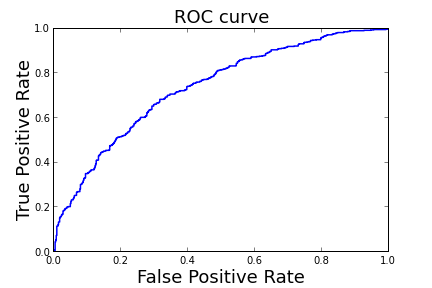
\includegraphics[height=6cm]{doc_en_01.png}

Need.... more .... power!

One thing that is missing, if you're predicting the next game based on the
previous few games, is that some teams may have just played a really tough
schedule, while other teams have played against much weaker competition.

We can solve for schedule difficulty by running another regression; this
one computes a power ranking, similar to the FIFA/CocaCola power ranking
for international soccer teams (there are power rankings for other sports
like college (american) football that may be familiar.)

Once we compute the power ranking (which creates a stack ranking of all of
the teams), we can add that power ranking as a feature to our model, then
rebuild it and re-validate it. The regression essentailly automated the
process of looking at relationships like "Well, team A beat team B and team
B beat team C, so A is probably better than C".

The output here will show the power ranking for various teams. This can be
useful to spot check the ranking, since if we rank Wiggan at 1.0 and
Chelsea at 0.0, something is likely wrong.

Note that because there isn't a strict ordering to the data (if team A
beats team B and team B beats team C, sometimes team C will then beat team
A) we sometimes fail to assign ordering to all of the teams (especially
where the data is sparse). For teams that we can't rank, we put them in the
middle (0.5).

Additionally, because the rankings for international teams are noisy and
sparse, we chunk the rankings into quartiles. So teams that have been
ranked will show up as 0, .33, .66, or 1.0.

Once we add this to the model, the performance generally improves significantly.

\begin{minted}[fontsize=\footnotesize]{python}
import power
reload(power)
reload(world_cup)
def points_to_sgn(p):
  if p > 0.1: return 1.0
  elif p < -0.1: return -1.0
  else: return 0.0
power_cols = [
  ('points', points_to_sgn, 'points'),
]

power_data = power.add_power(club_data, game_summaries, power_cols)
power_train = power_data.loc[power_data['points'] <> 1] 

# power_train = power_data
(power_model, power_test) = world_cup.train_model(
    power_train, match_stats.get_non_feature_columns())
print "\nRsquared: %0.03g, Power Coef %0.03g" % (
    power_model.prsquared, 
    math.exp(power_model.params['power_points']))

power_results = world_cup.predict_model(power_model, power_test, 
    match_stats.get_non_feature_columns())
power_y = [yval == 3 for yval in power_test['points']]
world_cup.validate(3, power_y, power_results['predicted'], baseline, 
                   compute_auc=True, quiet=False)

print_params(power_model, 8)

plt.plot([0, 1], [0, 1], '--', color=(0.6, 0.6, 0.6), label='Luck')
# Add the old model to the graph
world_cup.validate('old', y, results['predicted'], baseline, 
                   compute_auc=True, quiet=True)
plt.legend(loc="lower right")
plt.savefig('doc_en_02.png')
\end{minted}

\begin{verbatim}
New season 2014
New season 2013
QC check did not pass for 19 out of 20 parameters
Try increasing solver accuracy or number of iterations, decreasing alpha, or switch solvers
Could not trim params automatically due to failed QC check.  Trimming using trim_mode == 'size' will still work.
New season 2013
New season 2012
QC check did not pass for 24 out of 24 parameters
Try increasing solver accuracy or number of iterations, decreasing alpha, or switch solvers
Could not trim params automatically due to failed QC check.  Trimming using trim_mode == 'size' will still work.
New season 2012
New season 2011
QC check did not pass for 24 out of 24 parameters
Try increasing solver accuracy or number of iterations, decreasing alpha, or switch solvers
Could not trim params automatically due to failed QC check.  Trimming using trim_mode == 'size' will still work.
['Blackburn Rovers: 0.000', 'Real Betis: 0.000', 'D.C. United: 0.000',
'Celta de Vigo: 0.004', 'Deportivo de La Coru\xc3\xb1a: 0.009',
'Wolverhampton Wanderers: 0.021', 'Reading: 0.022', 'Real Zaragoza: 0.026',
'Real Valladolid: 0.044', 'Granada CF: 0.062', 'Queens Park Rangers:
0.073', 'Mallorca: 0.089', 'Aston Villa: 0.092', 'Bolton Wanderers: 0.102',
'Osasuna: 0.109', 'Espanyol: 0.112', 'Wigan Athletic: 0.124', 'Sunderland:
0.130', 'Rayo Vallecano: 0.138', 'Almer\xc3\xada: 0.145', 'Levante: 0.148',
'Elche: 0.154', 'Getafe: 0.170', 'Swansea City: 0.192', 'Southampton:
0.197', 'Norwich City: 0.206', 'Toronto FC: 0.211', 'Chivas USA: 0.218',
'West Ham United: 0.220', 'West Bromwich Albion: 0.224', 'Villarreal:
0.231', 'Stoke City: 0.255', 'Fulham: 0.274', 'Valencia: 0.296', 'Valencia
CF: 0.296', 'M\xc3\xa1laga: 0.305', 'Newcastle United: 0.342', 'Sevilla:
0.365', 'Columbus Crew: 0.366', 'Athletic Club: 0.386', 'Liverpool: 0.397',
'Everton: 0.417', 'Philadelphia Union: 0.466', 'Montreal Impact: 0.470',
'Chelsea: 0.530', 'Real Sociedad: 0.535', 'Tottenham Hotspur: 0.551',
'Arsenal: 0.592', 'Houston Dynamo: 0.593', 'FC Dallas: 0.612', 'Chicago
Fire: 0.612', 'Vancouver Whitecaps: 0.615', 'San Jose Earthquakes: 0.632',
'New England Revolution: 0.634', 'Atl\xc3\xa9tico de Madrid: 0.672',
'Colorado Rapids: 0.743', 'Barcelona: 0.759', 'Seattle Sounders FC: 0.781',
'New York Red Bulls: 0.814', 'Sporting Kansas City: 0.854', 'LA Galaxy:
0.882', 'Real Salt Lake: 0.922', 'Manchester City: 0.928', 'Real Madrid:
1.000', 'Manchester United: 1.000', 'Portland Timbers: 1.000'] 

Rsquared: 0.22, Power Coef 2.18
(3) Lift: 1.56 Auc: 0.791
    Base: 0.374 Acc: 0.708 P(1|t): 0.778 P(0|f): 0.667
    Fp/Fn/Tp/Tn p/n/c: 99/248/347/496 595/595/1190
Positive features
power_points      1.177169
is_home           0.787110
opp_op_corners    0.170848
expected_goals    0.058597
opp_cards         0.045538
pass_70           0.036267
avg_goals         0.035456
opp_avg_points    0.033857
dtype: float64

Dropped features
passes                0
op_pass_80            0
op_expected_goals     0
opp_shots_op_ratio    0
bad_passes            0
pass_ratio            0
opp_pass_op_ratio     0
shots                 0
dtype: float64

Negative features
opp_power_points     -0.540688
op_corners           -0.145918
opp_expected_goals   -0.055353
cards                -0.043555
opp_pass_70          -0.034997
opp_avg_goals        -0.034242
avg_points           -0.032748
opp_fouls            -0.022867
dtype: float64
(old) Lift: 1.42 Auc: 0.738
\end{verbatim}

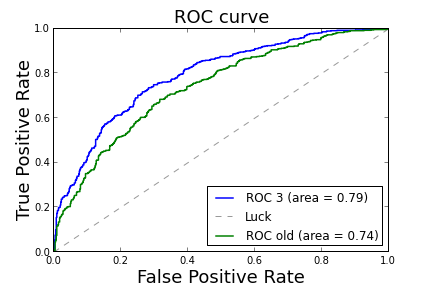
\includegraphics[height=6cm]{doc_en_02.png}


On to the world cup!

Now that we've got a model that we like, let's look at predicting the world
cup. We can build the same statistics (features) for the world cup games
that we did for the club games. In this case, however, we don't have the
targets; that is, we don't know who won (for some of the previous games, we
do know who won, but let's predict them all equally as if we didn't know).

\verb!features.get_wc_features()! will return build features from the world
cup games.

\begin{minted}[fontsize=\footnotesize]{python}
import world_cup
import features
reload(match_stats)
reload(features)
reload(world_cup)
wc_data = world_cup.prepare_data(features.get_wc_features(history_size))
wc_labeled = world_cup.prepare_data(features.get_features(history_size))
wc_labeled = wc_labeled[wc_labeled['competitionid'] == 4]
wc_power_train = game_summaries[game_summaries['competitionid'] == 4].copy()
\end{minted}

Predicting the world cup

Once we have the model and the features, we can start predicting.

Home Team Advantage

There are a couple of differences between the world cup and club data. For
one, while home team advantage is important in club games, who is really at
home? Is it only Brazil? What about other south american teams? Some models
give the 'is home' status to only Brazil, others give partial status to
other teams from the same continent, since historical data shows that teams
from the same continent tend to outperform.

We use a slightly modified model that is, however, somewhat subjective. We
assing a value to \verb!is_home! between 0.0 to 1.0 depending on the fan
support (both numbers and enthusiasm) that a team enjoys. This is a result
of noticing, in the early rounds, that the teams that had the more
entusiastic supporters did better. For example, Chile's fans were deafining
in support of their team, but Spain's fans barely showed up (Chile upset
spain 2-0). There were a number of other cases like this; many involving
south american sides, but many involving other teams that had sent a lot of
supporters (Mexico, for example). Some teams, like the USA, had a lot of
fans, but they were more reserved... they got a lower score. This factor
was set based on first-hand reports from the group games.

\begin{minted}[fontsize=\footnotesize]{python}
import pandas as pd
wc_home = pd.read_csv('wc_home.csv')

def add_home_override(df, home_map):
  for ii in xrange(len(df)):
    team = df.iloc[ii]['teamid']
    if team in home_map:
        df['is_home'].iloc[ii] = home_map[team]
    else:
        # If we don't know, assume not at home.
        df['is_home'].iloc[ii] = 0.0
        
home_override = {}
for ii in xrange(len(wc_home)):
    row = wc_home.iloc[ii]
    home_override[row['teamid']] = row['is_home']

# Add home team overrides.
add_home_override(wc_data, home_override)    
\end{minted}

World Cup Power Rankings

The lattice of teams playing eachother in the world cup is pretty
sparse. Many teams haven't played eachother for decades. Many European
teams rarely play South American ones, and even more rarely play Asian
ones. We can use the same technique as we did for the club games, but we
have to be prepared for failure.

We'll output the power rankings from the previous games. We should eyeball
them to make sure they make sense.

\begin{minted}[fontsize=\footnotesize]{python}
# When training power data, since the games span multiple competitions, 
# just set is_home to 0.5
#
# Otherwise when we looked at games from the 2010 world cup, we'd think 
# Brazil was still at home instead of South Africa.

wc_power_train['is_home'] = 0.5
wc_power_data = power.add_power(wc_data, wc_power_train, power_cols)

wc_results = world_cup.predict_model(power_model, wc_power_data, 
    match_stats.get_non_feature_columns())
\end{minted}

\begin{verbatim}
New season 2013
New season 2009
New season 6
QC check did not pass for 45 out of 50 parameters
Try increasing solver accuracy or number of iterations, decreasing alpha, or switch solvers
Could not trim params automatically due to failed QC check.  Trimming using trim_mode == 'size' will still work.
['Australia: 0.000', 'Serbia: 0.016', 'USA: 0.017', 'Cameroon: 0.035',
'Iran: 0.081', 'Croatia: 0.180', 'Nigeria: 0.204', "C\xc3\xb4te d'Ivoire:
0.244", 'Costa Rica: 0.254', 'Algeria: 0.267', 'Paraguay: 0.277',
'Honduras: 0.279', 'Slovakia: 0.281', 'Greece: 0.284', 'Switzerland:
0.291', 'Ecuador: 0.342', 'Uruguay: 0.367', 'Sweden: 0.386', 'Japan:
0.406', 'Mexico: 0.409', 'Chile: 0.413', 'Colombia: 0.438', 'England:
0.460', 'Belgium: 0.467', 'Ukraine: 0.470', 'Portugal: 0.487', 'Ghana:
0.519', 'South Korea: 0.532', 'France: 0.648', 'Spain: 0.736', 'Argentina:
0.793', 'Italy: 0.798', 'Brazil: 0.898', 'Netherlands: 0.918', 'Germany:
1.000'] 
\end{verbatim}


Predicting games

Now's the moment we've been waiting for. Let's predict some world cup games. Let's start with predicting the ones that have already happenned.

We will output 4 columns:

\verb!team_name!: Team we're predicting

\verb!op_team_name!: Team that the team we're predicting is playing against

\verb!predicted!: Precentage chance (we believe) that the team will win.

\verb!points!: If the game has been played, what actually happenned. (if
the game hasn't been played, we'll show a \verb!NaN! here). 3 points is a
win, 1 point is a draw, 0 points is a loss. Note that for games in the
knockout phase that went into penalty kicks, we'll mark that as a draw.

But wait! These predictions are different from the ones you published!

There are three reasons why the prediction numbers might be different from
the numbers you may have seen as published predictions:

We've updated our code several times to fix bugs and improve accuracy. Our
original model, for example, didn't account for extra time causing inflated
statistics.

Model building is non-deterministic. Since we pick a random subset of the
data to use as our training set, the results will change from run to
run. Sometimes fairly significantly.

When we predicted the round of 16, we used the trailing 3 games to predict
(since each team had played 3 games in the current world cup). For the
quarterfinals, we used the trailing 4 games; for the semis, 5, and for the
finals, we used all 6 [in this notebook, we use different ones at times,
please check]. The code below will predict based on the last 6 games; for
many teams, we don't have 6 games of history, and even if we do, that
history will be from previous world cups. To see a more apples-to-apples
comparison, set the \verb!history_size!  variable to 3 and rerun the
notebook.

\begin{minted}[fontsize=\footnotesize]{python}
pd.set_option('display.max_rows', 5000)
pd.set_option('display.max_columns', 500)
pd.set_option('display.width', 1000)

wc_with_points = wc_power_data.copy()
wc_with_points.index = pd.Index(
    zip(wc_with_points['matchid'], wc_with_points['teamid']))
wc_labeled.index = pd.Index(
    zip(wc_labeled['matchid'], wc_labeled['teamid']))
wc_with_points['points'] = wc_labeled['points']

wc_pred = world_cup.extract_predictions(wc_with_points, 
                                        wc_results['predicted'])

# Reverse our predictions to show the most recent first.
wc_pred.reindex(index=wc_pred.index[::-1])
# Show our predictions for the games that have already happenned.
print wc_pred
\end{minted}

\begin{verbatim}
        team_name   op_team_name  predicted       expected         winner  points
0       Argentina        Germany  46.070814        Germany             NA     NaN
1     Netherlands         Brazil  42.833863         Brazil             NA     NaN
2     Netherlands      Argentina  48.641542      Argentina           draw       1
3         Germany         Brazil  44.011593         Brazil        Germany       3
4      Costa Rica    Netherlands  14.442625    Netherlands           draw       1
5         Belgium      Argentina  18.596031      Argentina      Argentina       0
6        Colombia         Brazil  23.890421         Brazil         Brazil       0
7         Germany         France  75.116349        Germany        Germany       3
8             USA        Belgium  32.400646        Belgium        Belgium       0
9     Switzerland      Argentina  19.272768      Argentina      Argentina       0
10        Algeria        Germany   5.926496        Germany        Germany       0
11        Nigeria         France   8.694729         France         France       0
12         Greece     Costa Rica  40.448104     Costa Rica           draw       1
13         Mexico    Netherlands  20.402491    Netherlands    Netherlands       0
14        Uruguay       Colombia  46.480264       Colombia       Colombia       0
15          Chile         Brazil  26.574916         Brazil           draw       1
16        Germany            USA  91.980986        Germany        Germany       3
17          Ghana       Portugal  49.051707       Portugal       Portugal       0
18    Switzerland       Honduras  60.223070    Switzerland    Switzerland       3
19         France        Ecuador  84.538857         France           draw       1
20      Argentina        Nigeria  88.491450      Argentina      Argentina       3
21  Côte d'Ivoire         Greece  61.074502  Côte d'Ivoire         Greece       0
22        Uruguay          Italy  32.685428          Italy        Uruguay       3
23        England     Costa Rica  63.457326        England           draw       1
24         Brazil       Cameroon  94.788074         Brazil         Brazil       3
25         Mexico        Croatia  78.020214         Mexico         Mexico       3
26          Spain      Australia  90.521542          Spain          Spain       3
27          Chile    Netherlands  28.342133    Netherlands    Netherlands       0
28       Portugal            USA  65.457259       Portugal           draw       1
29        Algeria    South Korea  17.376285    South Korea        Algeria       3
30          Ghana        Germany  14.588539        Germany           draw       1
31           Iran      Argentina   5.193843      Argentina      Argentina       0
32        Ecuador       Honduras  53.848926        Ecuador        Ecuador       3
33         France    Switzerland  78.659381         France         France       3
34     Costa Rica          Italy  24.836756          Italy     Costa Rica       3
35         Greece          Japan  44.355013          Japan           draw       1
36        England        Uruguay  61.012694        England        Uruguay       0
37        Croatia       Cameroon  40.212875       Cameroon        Croatia       3
38          Chile          Spain  42.624474          Spain          Chile       3
39    Netherlands      Australia  93.535889    Netherlands    Netherlands       3
40         Mexico         Brazil  20.372064         Brazil           draw       1
41            USA          Ghana  39.500993          Ghana            USA       3
42        Nigeria           Iran  53.813244        Nigeria           draw       1
43       Portugal        Germany  15.337884        Germany        Germany       0
44       Honduras         France  22.953848         France         France       0
45        Ecuador    Switzerland  59.987076        Ecuador    Switzerland       0
46          Japan  Côte d'Ivoire  51.528885          Japan  Côte d'Ivoire       0
47          Italy        England  68.767968          Italy          Italy       3
48     Costa Rica        Uruguay  45.347946        Uruguay     Costa Rica       3
49      Australia          Chile  19.487987          Chile          Chile       0
50    Netherlands          Spain  60.493928    Netherlands    Netherlands       3
51       Cameroon         Mexico  30.018950         Mexico         Mexico       0
52        Croatia         Brazil   6.268704         Brazil         Brazil       0
53          Spain    Netherlands  35.602227    Netherlands          Spain       3
54        Germany        Uruguay  76.467450        Germany        Germany       3
55          Spain        Germany  29.438134        Germany          Spain       3
56    Netherlands        Uruguay  71.342186    Netherlands    Netherlands       3
57          Spain       Paraguay  83.007655          Spain          Spain       3
58        Germany      Argentina  42.635127      Argentina        Germany       3
59          Ghana        Uruguay  41.784682        Uruguay           draw       1
60         Brazil    Netherlands  60.821972         Brazil    Netherlands       0
61       Portugal          Spain  23.464891          Spain          Spain       0
62          Japan       Paraguay  61.278000          Japan           draw       1
63          Chile         Brazil  24.459600         Brazil         Brazil       0
64       Slovakia    Netherlands  12.082967    Netherlands    Netherlands       0
65         Mexico      Argentina  17.626748      Argentina      Argentina       0
66        England        Germany  20.763176        Germany        Germany       0
67          Ghana            USA  71.310871          Ghana          Ghana       3
68    South Korea        Uruguay  45.148588        Uruguay        Uruguay       0
69         Brazil       Portugal  81.610878         Brazil           draw       1
70        Germany          Ghana  81.621494        Germany        Germany       3
71         Serbia      Australia  38.204905      Australia      Australia       0
72  Côte d'Ivoire         Brazil  10.186423         Brazil         Brazil       0
73      Australia          Ghana  23.702414          Ghana           draw       1
74          Japan    Netherlands  10.773998    Netherlands    Netherlands       0
75         Serbia        Germany   4.731113        Germany         Serbia       3
76         Mexico         France  42.801515         France         Mexico       3
77    South Korea      Argentina  15.255040      Argentina      Argentina       0
78    Switzerland          Spain  18.747704          Spain    Switzerland       3
79       Portugal  Côte d'Ivoire  65.031075       Portugal           draw       1
80       Paraguay          Italy  12.288896          Italy           draw       1
81      Australia        Germany   7.395354        Germany        Germany       0
82          Ghana         Serbia  83.682899          Ghana          Ghana       3
83            USA        England  34.763699        England           draw       1
84         France          Italy  28.651132          Italy           draw       1
85       Portugal        Germany  14.833907        Germany        Germany       0
86         France       Portugal  72.141913         France         France       3
87          Italy        Germany  33.364112        Germany          Italy       3
88         France         Brazil  22.742882         Brazil         France       3
89       Portugal        England  49.550454        England           draw       1
90        Ukraine          Italy  28.378865          Italy          Italy       0
91      Argentina        Germany  46.801014        Germany           draw       1
92         France          Spain  47.126654          Spain         France       3
93          Ghana         Brazil   9.144470         Brazil         Brazil       0
94        Ukraine    Switzerland  62.637340        Ukraine           draw       1
95      Australia          Italy   8.365416          Italy          Italy       0
96    Netherlands       Portugal  70.231295    Netherlands       Portugal       0
97        Ecuador        England  34.379086        England        England       0
98         Mexico      Argentina  29.233199      Argentina      Argentina       0
99         Sweden        Germany  10.914079        Germany        Germany       0
\end{verbatim}

References

[1] \url{http://googlecloudplatform.blogspot.de/2014/07/google-cloud-platform-goes-8-for-8-in-soccer-predictions.html}

[2] \url{https://github.com/GoogleCloudPlatform/ipython-soccer-predictions}

[3] \url{http://nbviewer.ipython.org/github/GoogleCloudPlatform/ipython-soccer-predictions/blob/master/predict/wc-final.ipynb}


\end{document}
